\documentclass[11pt,a4paper]{article}
\usepackage[utf8]{inputenc}
\usepackage[margin=22mm]{geometry}
\usepackage{amsmath,amssymb}
\usepackage{graphicx}
\usepackage{booktabs}
\usepackage{array,tabularx}
\usepackage{float}
\usepackage{xcolor}
\usepackage{hyperref}
\hypersetup{colorlinks=true,linkcolor=blue!45!black,urlcolor=blue!50!black,citecolor=blue!45!black}
\newcolumntype{Y}{>{\raggedright\arraybackslash}X}
\setlength{\emergencystretch}{2em}
\setlength{\tabcolsep}{4pt}
\renewcommand{\arraystretch}{1.08}
\graphicspath{{figures/}}
\title{\textbf{Reinforcement Learning for Energy-Efficient Routing}\\[0.3em]\large Short Project Report}
\author{}
\date{}
\begin{document}
\maketitle
\begin{abstract}
This project studies routing in a simulated software-defined wireless sensor network. A controller learns next-hop choices using energy, congestion and link reliability as objectives. Q-learning, SARSA, Monte Carlo control and linear Q-function approximation are evaluated. The harder route task shows improving training return, and DOS Q-learning has higher mean delivery than re-planned shortest path in the tested outage scenarios. These network differences are descriptive, not statistically established. All network metrics are estimates from an analytical simulator.
\end{abstract}

\section{Problem Understanding and Literature Review}
Sensor nodes send data to a gateway, sometimes through battery-powered relays. A short route can overuse the same relays, encounter congestion or use unreliable links. The objective is to select forwarding routes that deliver data while considering energy, buffer load and link quality. The study uses a simulated controller, not a physical deployment.

RL learns actions through interaction and feedback. Q-learning estimates action values using the best estimated next value \cite{watkins}; SARSA uses the next action selected by its policy \cite{sutton}. The project also uses multi-objective routing ideas motivated by Godfrey et al. \cite{godfrey}, and distance-based reward shaping \cite{ng}. The background paper is a reference for the problem area.

\section{MDP Formulation and Reward Design}
A route episode starts at a source and ends when the packet reaches the gateway or fails. Its main components are:
\begin{table}[H]
\centering\small
\caption{Routing decision process.}
\begin{tabularx}{\linewidth}{@{}lY@{}}\toprule
\textbf{Element} & \textbf{Project definition}\\\midrule
Agent and environment & Controller choosing next hops in a simulated relay network.\\
State & Current relay ID. Energy, load and history affect outcomes but are not included in this key.\\
Action & Eligible neighbouring relay, or the gateway when directly reachable.\\
Transition & A successful hop advances the packet; exhausted link attempts, low energy, a dead end, a loop or a hop limit can end the route.\\
Goal & Reach the gateway while considering energy, congestion and link quality.\\\bottomrule
\end{tabularx}
\end{table}
The relay-only key keeps the table manageable, but different network conditions can share the same key; it is not proven to be a complete Markov state. A separate expanded-state experiment captures more route context, but exact snapshot keys did not recur during its evaluation, limiting tabular generalisation.

The model estimates per-attempt packet reception ratio (PRR) from a distance-based radio model. With per-attempt success probability $p$ and at most $R$ independent attempts, hop success is $1-(1-p)^R$. The flow model uses the corrected expected attempt count $\sum_{k=0}^{R-1}(1-p)^k$. This is an analytical approximation, not a packet-level measurement.

\subsection{Rewards and objective selection}
Each action has three reward components: energy favours a relatively well-powered receiver; buffer/load favours available capacity; link reward is the estimated link PRR. For sender $i$ and receiver $j$:
\begin{equation*}
r_E=\tfrac12(1+e_j-e_i),\qquad
r_Q=\tfrac12(1+(1-q_j)-\ell_i),\qquad r_L=p_{ij}.
\end{equation*}
Here $e$ is normalised energy, $q_j$ is receiver buffer occupancy, $\ell_i$ is sender load and $p_{ij}$ is estimated PRR. The gateway has special reward conventions. Reaching it earns a terminal bonus; failures normally incur a penalty.

Dynamic objective selection (DOS) maintains separate objective values. The default value-based rule selects the objective with the highest available estimated Q-value, then selects an action using that objective. Weighted-sum Q-learning instead combines the reward components into one weighted reward and learns a single Q-value.

Potential-based shaping provides an additional progress signal \cite{ng}:
\begin{equation*}
F(s,s')=\gamma\Phi(s')-\Phi(s),\qquad
\Phi(s)=1-\frac{d(s,G)}{d_{\max}}.
\end{equation*}
Here $d(s,G)$ is distance to the gateway, and terminal potential is zero. This signal is not necessarily positive for every closer step, and the experiment does not establish a shaping advantage.

\section{Working Implementation}
The Python implementation trains agents on route episodes using epsilon-greedy exploration and tests them greedily. A default breadth-first-search/geographic action restriction favours gateway progress but does not guarantee loop-free behaviour in every fallback. An episode can terminate immediately without a failure update when no initial action exists.
\begin{table}[H]
\centering\small
\caption{Implemented learning methods.}
\begin{tabularx}{\linewidth}{@{}lY@{}}\toprule
\textbf{Method} & \textbf{How it learns}\\\midrule
DOS Q-learning & Updates each objective using reward and the best estimated next-action value.\\
Weighted-sum Q-learning & Learns one Q-value from a weighted combination of objective rewards.\\
SARSA & Updates using the next action actually selected by its current policy.\\
Monte Carlo control & Waits for the episode to end and updates using its observed discounted return.\\
Linear Q approximation & Estimates objective Q-values from features such as energy, queue, load and PRR, and updates feature weights.\\\bottomrule
\end{tabularx}
\end{table}
After training, the policy is evaluated in the network simulator. Routes can be replanned as conditions change, but learned Q-values remain frozen. Main code is in \texttt{dos\_rl/mdp.py}, \texttt{dos\_rl/agents/}, \texttt{dos\_rl/trainer.py} and \texttt{dos\_rl/network\_sim.py}. A simulator-backed browser demonstration is in \texttt{visualization/}.

\begin{table}[H]
\centering\small
\caption{Default network settings. Individual experiments vary these settings.}
\begin{tabularx}{\linewidth}{@{}lY@{}}\toprule
\textbf{Parameter} & \textbf{Setting}\\\midrule
Network & 30 relays, 1,500 $\times$ 1,500 m area, nominal 450 m range.\\
Traffic and battery & Five sources at 10 packets/s/source; 5 J nominal battery per relay.\\
Packet, duration, queue & 512 bits; 200 simulated seconds; analytical queue capacity 20.\\
ARQ and network RL & Up to 3 attempts; $\alpha=0.30$, $\gamma=0.85$, $\epsilon=0.30$.\\\bottomrule
\end{tabularx}
\end{table}

\section{Results and Interpretation}
Results use the corrected simulator outputs in \texttt{arq\_fixed\_suite/}. Packet delivery ratio (PDR) is the estimated fraction of offered packets reaching the gateway; delay and energy are also model estimates. PDR/W is the per-run PDR fraction divided by average network power, then averaged across runs. It is not network lifetime.

\subsection{Learning and comparison of RL methods}
Each learner was trained for 3,000 route episodes per seed and evaluated on 30 independently sampled test episodes per seed across eight seeds. Test episodes use a separate random stream, but share their agent's training topology. Route success is not the same metric as network PDR.
\begin{table}[H]
\centering\small
\caption{Default route task: mean greedy test performance across eight seeds.}
\begin{tabularx}{\linewidth}{@{}Yrr@{}}\toprule
\textbf{Learner} & \textbf{Route success} & \textbf{Test return}\\\midrule
DOS Q-learning & 93.3\% & 10.48\\
Weighted-sum Q-learning & 94.2\% & 10.67\\
SARSA & 95.0\% & 10.84\\
Monte Carlo control & 95.0\% & 10.85\\
Linear Q approximation & 92.9\% & 10.46\\\bottomrule
\end{tabularx}
\end{table}
All methods perform well on this task; the descriptive means do not establish a significant ranking. The harder cold-start task gives a clearer view of learning, as shown in Table~\ref{tab:cold} and Figure~\ref{fig:cold}. Training uses exploration; the separate tests are greedy.
\begin{table}[H]
\centering\small
\caption{Harder task: 10 seeds, 1,500 training and 30 test episodes per seed. Early and late values are mean training returns.}
\label{tab:cold}
\begin{tabularx}{\linewidth}{@{}Yrrr@{}}\toprule
\textbf{Learner} & \textbf{Early return} & \textbf{Late return} & \textbf{Test success}\\\midrule
DOS Q-learning & $-3.30$ & 1.38 & 82.0\%\\
Weighted-sum Q-learning & $-2.96$ & 0.82 & 79.7\%\\\bottomrule
\end{tabularx}
\end{table}
\begin{figure}[H]
\centering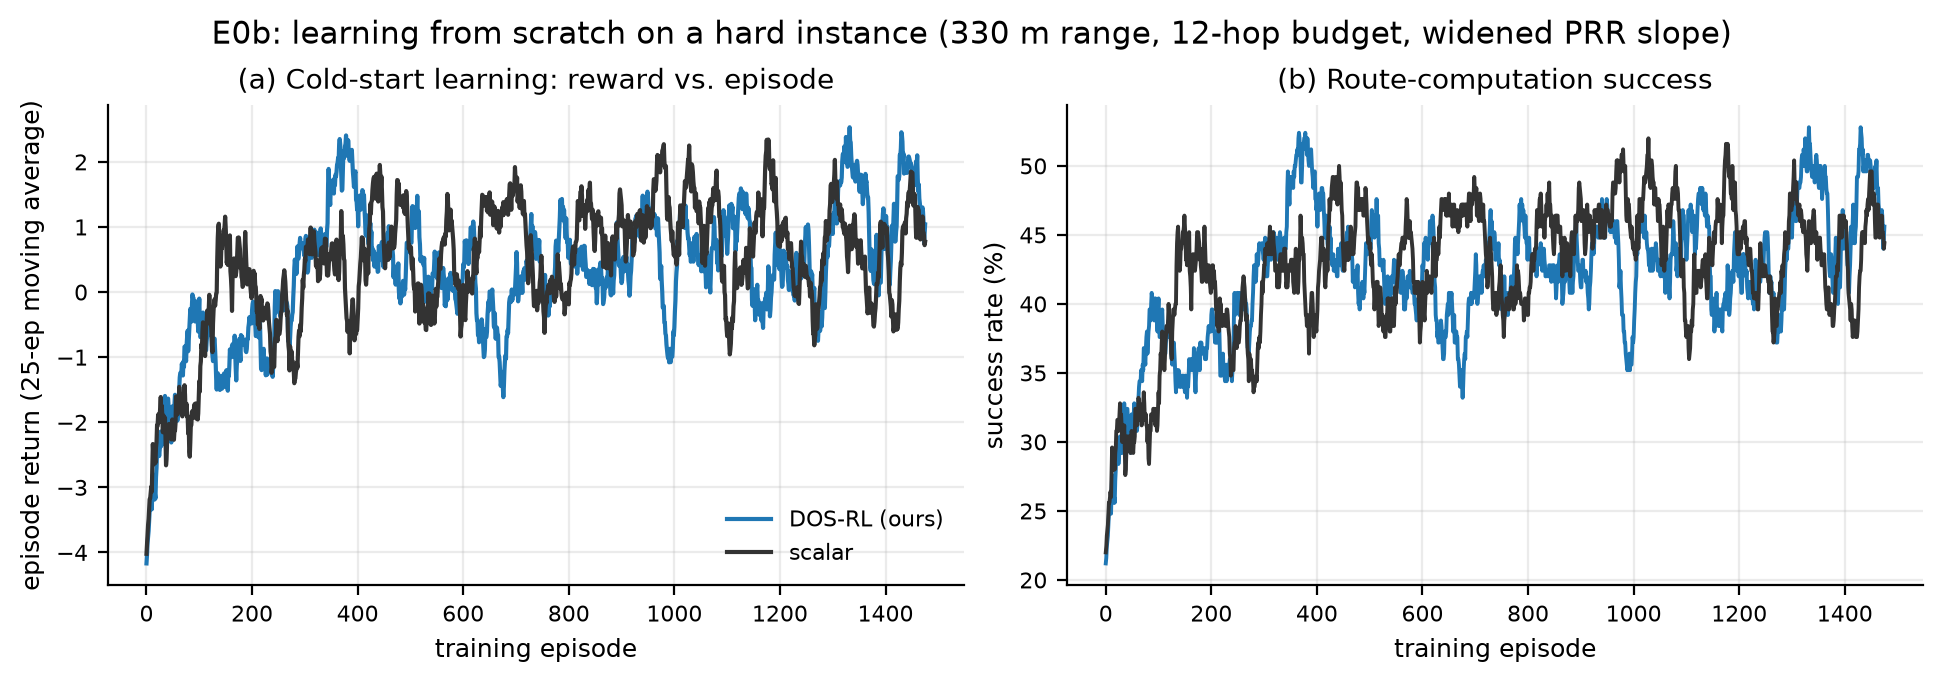
\includegraphics[width=\linewidth]{e0b_coldstart.png}
\caption{Harder task: training return and route success versus episodes; curves are seed averages smoothed over 25 episodes. ``scalar'' means weighted-sum Q-learning.}
\label{fig:cold}
\end{figure}
Both agents improve from the early to the late training window, consistent with learning. This does not establish that DOS is statistically superior to weighted-sum Q-learning.

\subsection{RL and a conventional routing policy}
The following matched experiments compare DOS Q-learning with re-planned shortest path. The latter is a non-RL baseline. In the offered-load experiment, five sources are used and results are means over ten deployments for each traffic setting.
\begin{table}[H]
\centering\small
\caption{Offered load: DOS Q-learning versus re-planned shortest path.}
\label{tab:load}
\begin{tabularx}{\linewidth}{@{}Yrrrr@{}}\toprule
\textbf{Packets/s/source} & \textbf{DOS PDR} & \textbf{Shortest PDR} & \textbf{DOS delay} & \textbf{Shortest delay}\\
& (\%) & (\%) & (ms) & (ms)\\\midrule
10 & 91.58 & 91.63 & 36.92 & 37.21\\
20 & 90.99 & 91.03 & 44.74 & 45.52\\
30 & 89.46 & 89.04 & 54.65 & 56.43\\
45 & 87.73 & 87.87 & 67.54 & 67.21\\
60 & 84.14 & 83.81 & 81.90 & 84.99\\
80 & 82.60 & 82.12 & 82.71 & 85.26\\\bottomrule
\end{tabularx}
\end{table}
\begin{figure}[H]
\centering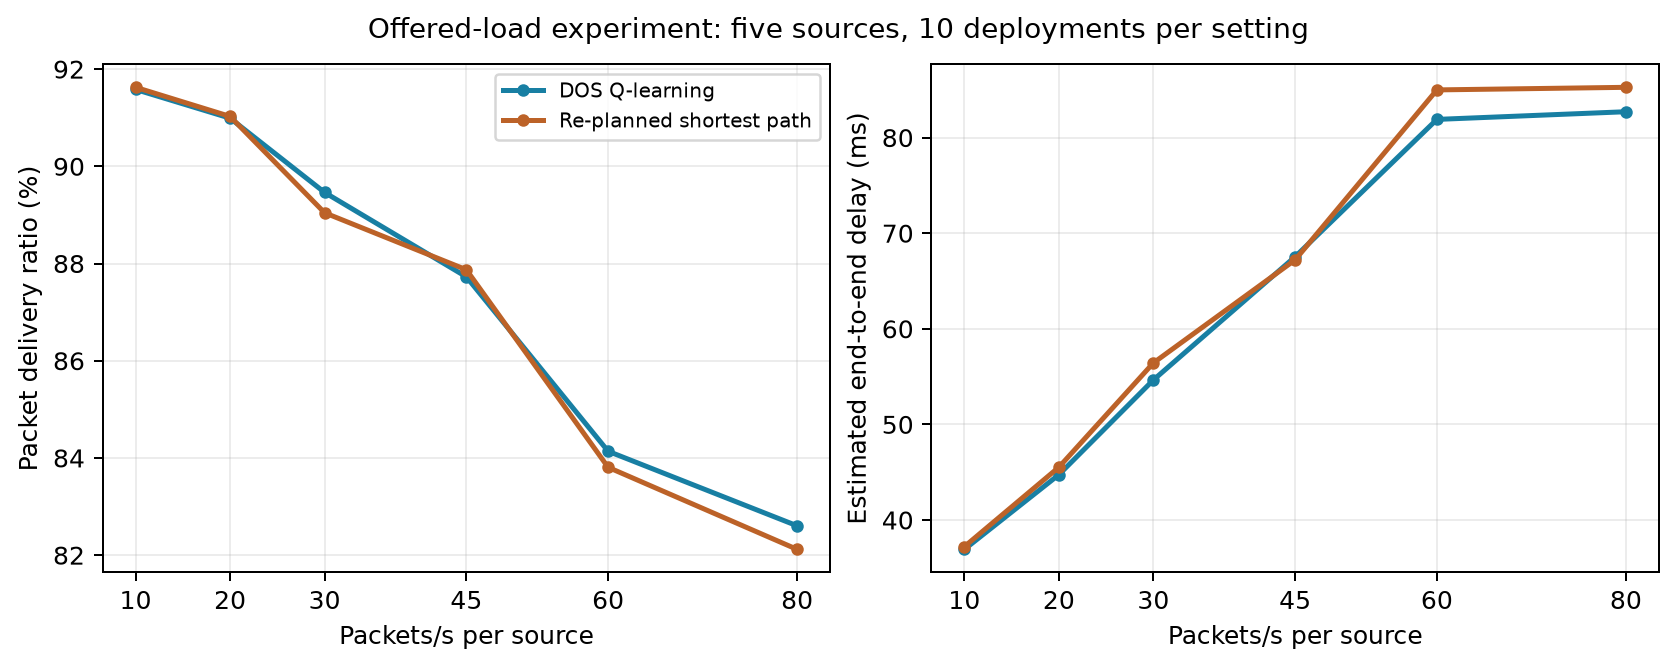
\includegraphics[width=\linewidth]{offered_load.png}
\caption{Delivery and estimated delay as offered load changes. Each point is a mean over ten deployments.}
\label{fig:load}
\end{figure}
At the two highest displayed loads, DOS has higher mean PDR and lower mean delay than shortest path. At other loads the ordering differs and the curves are close. These are descriptive results, not evidence of a statistically established advantage.

The temporary outage experiment offers another view of robustness. Post-onset PDR includes both the outage and the recovery period. All policies are evaluated on eight paired deployments; routes may be replanned but Q-values are frozen.
\begin{table}[H]
\centering\small
\caption{Temporary link-outage results: mean post-onset PDR.}
\label{tab:outage}
\begin{tabularx}{\linewidth}{@{}Yrrrr@{}}\toprule
\textbf{Links unavailable} & \textbf{DOS} & \textbf{Shortest} & \textbf{Difference} & \textbf{Wilcoxon $p$}\\\midrule
0\% & 91.55\% & 90.48\% & $+1.07$ pp & ---\\
20\% & 75.06\% & 72.19\% & $+2.87$ pp & 0.109\\
40\% & 74.12\% & 69.25\% & $+4.87$ pp & 0.078\\\bottomrule
\end{tabularx}
\end{table}
\begin{figure}[H]
\centering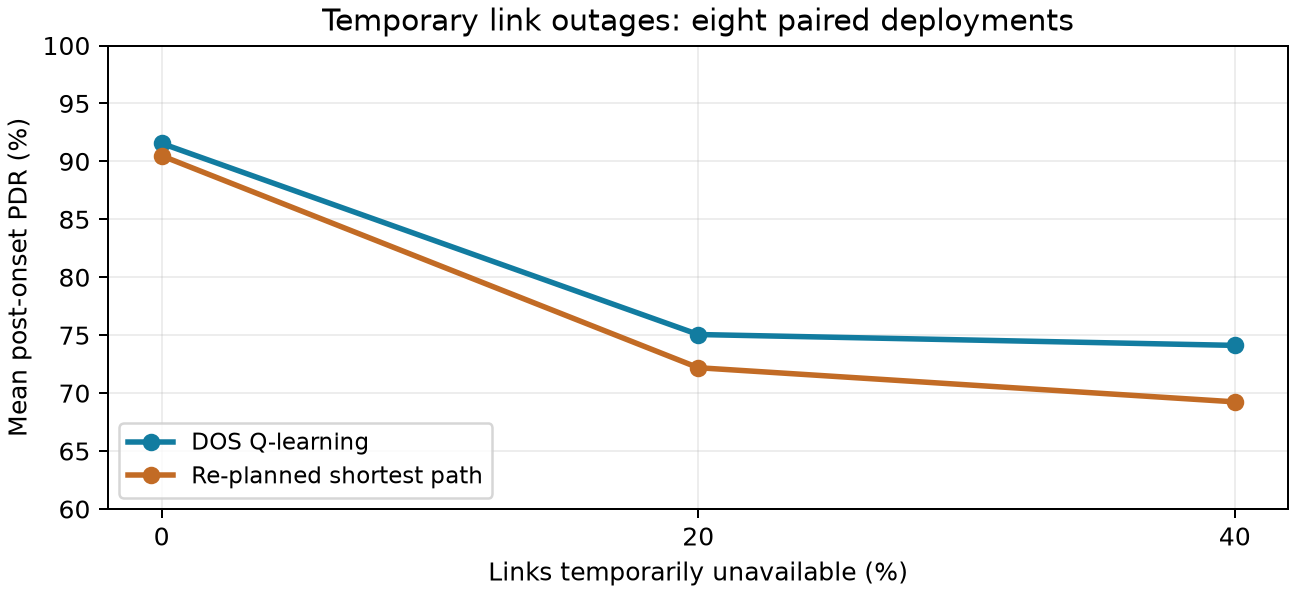
\includegraphics[width=0.85\linewidth]{link_outage.png}
\caption{Mean post-onset PDR during link-failure experiments, including recovery. The vertical axis starts at 60\%; paired tests are in Table~\ref{tab:outage}.}
\label{fig:outage}
\end{figure}
DOS has higher mean delivery in both tested outage conditions, suggesting a possible scenario-specific benefit. However, neither paired comparison meets the conventional 0.05 threshold; the sample is small, and no general superiority is established.

In a separate matched deployment battery, the RL agents were retrained for each topology. DOS again has slightly higher mean PDR and PDR/W than shortest path, but higher mean delay; the paired PDR test is not significant.
\begin{table}[H]
\centering\small
\caption{Retrained deployment battery: 30 matched deployments.}
\begin{tabularx}{\linewidth}{@{}Yrrrr@{}}\toprule
\textbf{Policy} & \textbf{PDR} & \textbf{Delay (ms)} & \textbf{PDR/W} & \textbf{Energy (J)}\\\midrule
DOS Q-learning & 87.15\% & 62.46 & 22.02 & 8.65\\
Re-planned shortest path & 86.68\% & 61.47 & 21.60 & 8.76\\\bottomrule
\end{tabularx}
\end{table}
The mean paired PDR difference is $+0.46$ percentage points (Wilcoxon $p=0.325$); it does not establish a PDR advantage.

\subsection{Parameter change and limitations}
Changing learning rate tests the effect of an RL design parameter. This sweep uses a relay-plus-energy/buffer-bin state; PDR difference is measured against re-planned shortest path.
\begin{table}[H]
\centering\small
\caption{Learning-rate sweep: six seeds, 2,500 training episodes per seed.}
\begin{tabularx}{\linewidth}{@{}lrrr@{}}\toprule
\textbf{Learning rate} & \textbf{Final training return} & \textbf{PDR difference} & \textbf{Approx. 95\% half-width}\\\midrule
0.02 & 10.36 & $-0.02$ pp & 2.08 pp\\
0.30 & 10.32 & $+1.41$ pp & 1.34 pp\\\bottomrule
\end{tabularx}
\end{table}
The higher learning rate has a larger descriptive PDR difference, but the intervals overlap; a reliable improvement is not established. A separate shaping ablation likewise did not establish a shaping advantage.

The compact state omits important evolving network variables. The simulator uses analytical radio, queue and flow models; training and network evaluation also differ in attempt accounting. Results depend on the selected scenarios and sample sizes, and are not proof of physical-network performance. Future work could use richer, generalisable states and packet-level or real-network testing.

\subsection{Conclusion}
The implementation learns multi-objective forwarding decisions and evaluates several RL methods. Results show learning on the harder route task and favourable mean PDR for DOS in the tested outages, while also showing that differences against shortest path are uncertain and scenario-dependent.

\begingroup\small
\begin{thebibliography}{9}\setlength{\itemsep}{0pt}
\bibitem{godfrey} D. Godfrey et al., ``An Energy-Efficient Routing Protocol with Reinforcement Learning in Software-Defined Wireless Sensor Networks,'' \emph{Sensors}, 23, 8435, 2023. \url{https://doi.org/10.3390/s23208435}.
\bibitem{watkins} C. J. C. H. Watkins and P. Dayan, ``Q-learning,'' \emph{Machine Learning}, 8, 279--292, 1992. \url{https://doi.org/10.1007/BF00992698}.
\bibitem{sutton} R. S. Sutton and A. G. Barto, \emph{Reinforcement Learning: An Introduction}, 2nd ed., MIT Press, 2018.
\bibitem{ng} A. Y. Ng, D. Harada and S. Russell, ``Policy Invariance Under Reward Transformations,'' \emph{ICML}, 1999.
\end{thebibliography}\endgroup
\end{document}
